\providecommand{\muh}{\hat{\mu}}
\providecommand{\yh}{\hat{y}}

\chapter{\label{chap:intro} Introduction}

% Motivation.1: information summarization.
One of the most exciting applications of natural language processing ahead of us is the development of systems that will be able to \textit{summarize information} for us.
For example, we will one day be able to rely on 
text summarization (TS) systems to condense the most salient information from one or more related articles into as few words as necessary (\reffig{intro:overview}(a)).
We will be be able to get targeted summaries through open-ended question answering systems (OQA) (\reffig{intro:overview}(b)).
Finally, knowledge base population (KBP) systems  will be able to read large document troves (or the Internet) and present succinct, structured, summaries about the people and organizations mentioned within (\reffig{intro:overview}(c)).

\begin{figure}
  \centering
  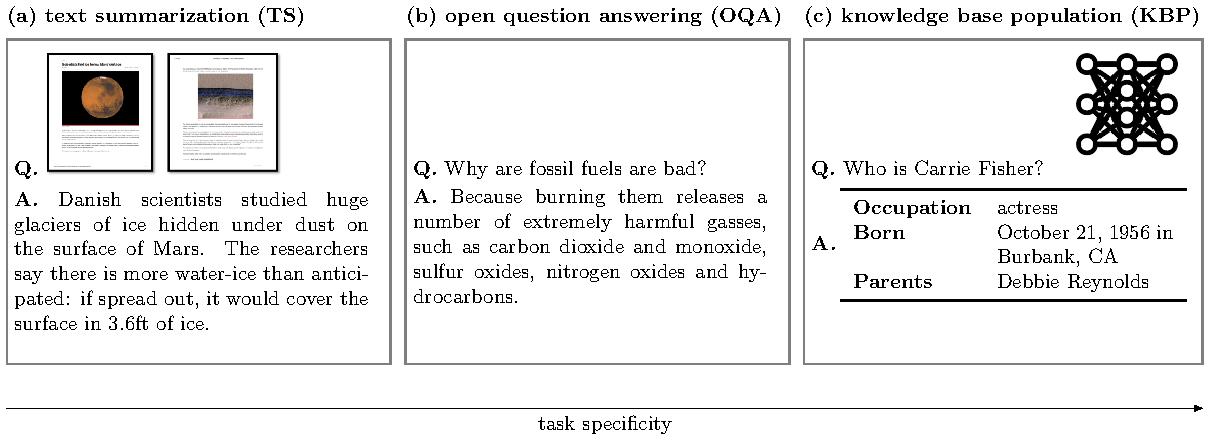
\includegraphics[width=\textwidth]{figures/overview}

  \caption[Overview of some information summarization tasks]{\label{fig:intro:overview} An overview of some information summarization tasks, listed in increasing specificity:
  (a) Text summarization: seeks to identify the most salient information contained within one (or more) article(s) and describe this information in as few words as necessary.
  (b) Open-response question answering: provides very-targeted summaries that address a specific question.
  (c) Knowledge base population: reads documents from a large corpus and generates linked entity-centric summaries for every person and organization mentioned within.
  }
\end{figure}

% Motivation.2: A brief history of work in the area
Indeed, this broad vision of summarization has been the goal of many natural language processing systems dating as far back as the 1950s~\citep{luhn1958automatic}.
Research has shown that having access to document summaries significantly improves user satisfaction and their ability to complete fact-gathering tasks~\citep{mani1999tipster, mckeown2005summaries}. 
Building these systems, however, remains a challenge.
Today, we are seeing a resurgence in interest in automatic summarization systems, with over 150 papers published at top NLP conferences in just the last year (2017--18).

% Motivation.3: Measurement is broken
Still, despite years of effort, it is unclear whether we are actually making forward progress on these tasks.
\citet{brandow1995automatic} conducted a large scale human evaluation of different summarization systems and found that the baseline of simply taking the lead-paragraph significantly outperformed automatic systems. 
Ten years later, \citet{passonneau2005applying} report that half of the systems participating in the DUC-2005 summarization challenge did worse than the baseline.
Even today, we find that recent ``state-of-the-art'' neural network based summarization systems fare poorly on human evaluations of language quality relative to simpler extractive systems.
While there are many reasons for thsi slow progress, we believe that the lack of an effective evaluation methodology remains one of the most important ones.

% Our contribution.
The ultimate goal of this thesis is to enable the development of better information summarization systems by addressing systemic problems in how we evaluate them.
In this work, we attribute the inherent \textit{incompleteness} of existing evaluation datasets as the key bottleneck to reliably measuring the performance of summarization systems.
We posit that collecting on-demand human feedback is fundamental to obtaining meaningful measures of system quality by resolving this incompleteness.
Our key technical contribution is applying techniques from statistical estimation to reliably integrate human feedback in a cost-effective manner.

\begin{figure}
  \centering
  \begin{subfigure}{0.25\textwidth}
  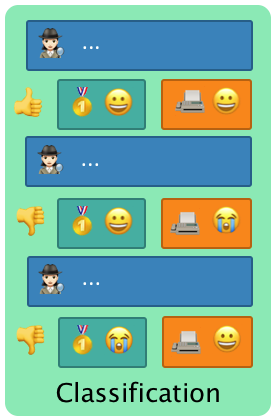
\includegraphics[width=\textwidth]{figures/incompleteness-classification}
  \end{subfigure} 
  \begin{subfigure}{0.25\textwidth}
  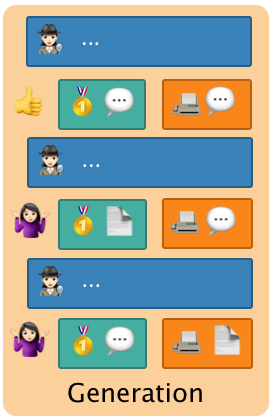
\includegraphics[width=\textwidth]{figures/incompleteness-generation}
  \end{subfigure}
  \caption[Complete and incomplete evaluation sets]{\label{fig:intro:evaluation-data} 
  Much of our evaluation methodology relies on a representative evaluation dataset that contains paired inputs and outputs.
  (a) When the outputs belong to a closed class, such as in classification tasks, it is easy to judge the output of a system and evaluate its performance.
  (b) On the other hand, in the summarization tasks we are interested in, there are many possible correct answers that are not represented in the evaluation data. In this sense, the evaluation data is \textit{incomplete}.
  }
\end{figure}
\section{The incompleteness of static evaluation sets}
At its core, the prevalent evaluation methodology today relies on a evaluation dataset that contains pairs of query inputs and expected outputs (\reffig{evaluation-data}).
On classification problems, e.g.\ sentiment classification or topic identification, the output typically belongs to a small closed class (e.g.\ positive, neutral or negative sentiment).
When a system also predicts an output belonging to this closed class, it is very easy to say whether or not the system made a mistake.
Thus, in these settings, we can measure the quality of different systems on the classification task by simply collecting a sufficiently large evaluation dataset.\footnote{%
Of course, care must be taken to ensure the evaluation dataset collected is reflective of the end-goal for the task.}

Unfortunately, in the summarization tasks we've seen above, the desired output is not simply a class label but rather an arbitrary piece of text (e.g.\ for TS and OQA) or an arbitrarily large collection of facts (e.g.\ for KBP).
The assumption that there exists a unique knowable correct output simply does not hold.
In this sense, the dataset is \textit{incomplete}: it either does not contain every possible correct answer or element.
Let's look at some examples of how incompleteness manifests in practice and what its consequences on evaluation could be.

\begin{figure}
  \centering
  \begin{subfigure}{0.65\textwidth}
    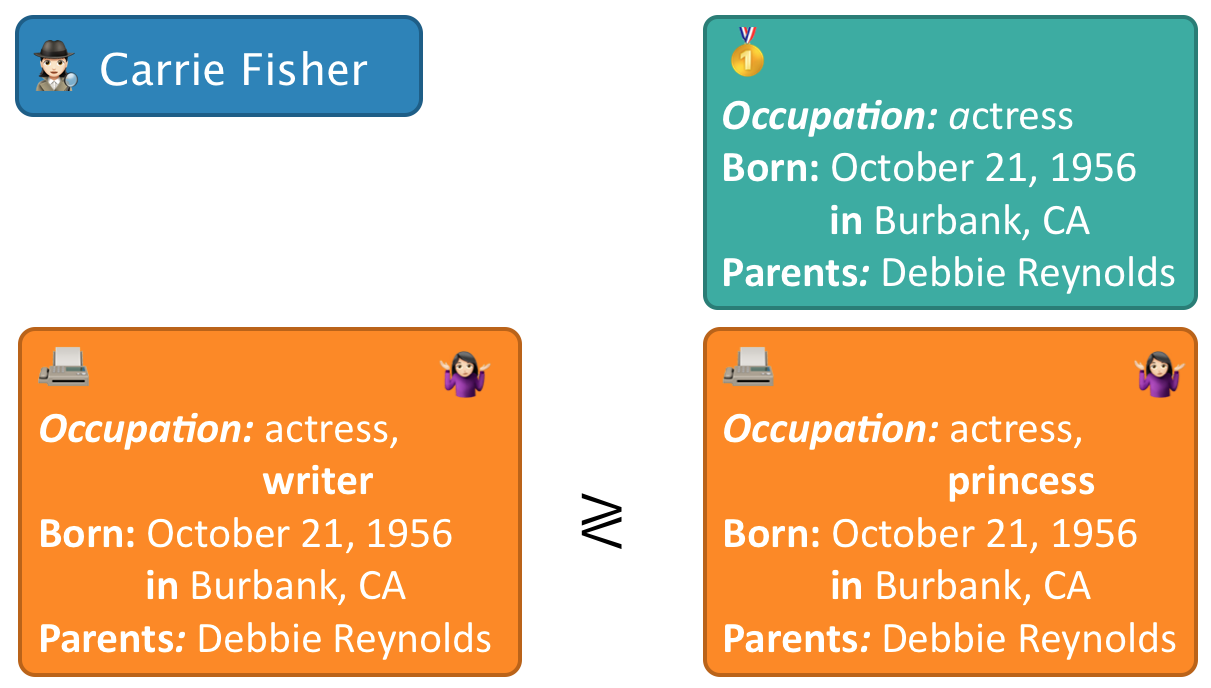
\includegraphics[width=\textwidth]{figures/example-kbp}
    \caption{\label{fig:intro:example-kbp} Knowledge base population.}
  \end{subfigure} \\
  \begin{subfigure}{0.65\textwidth}%
    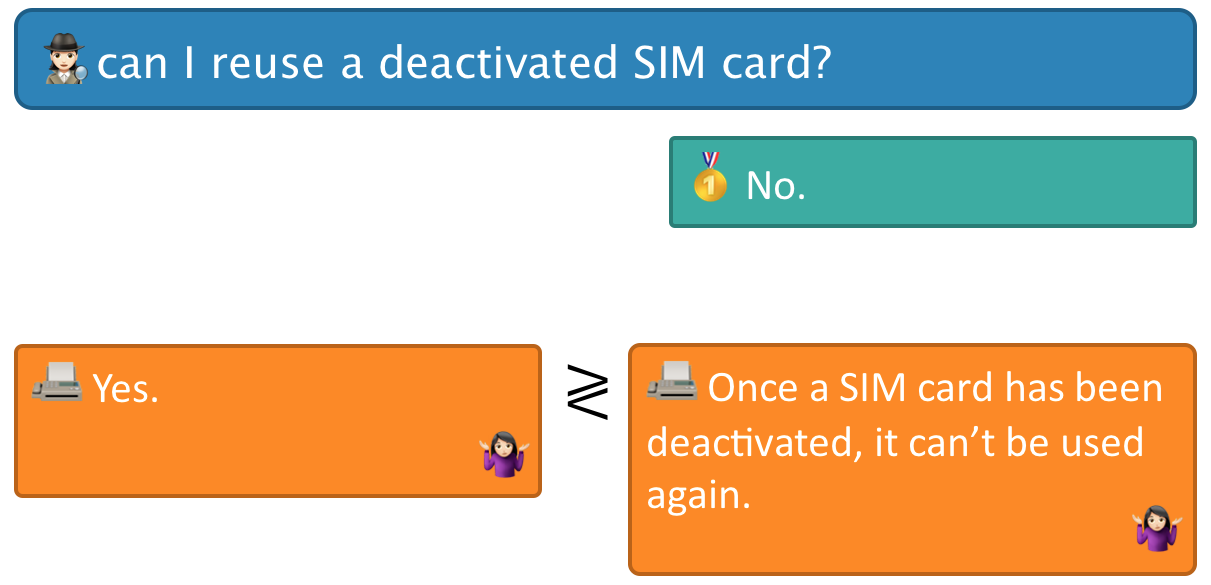
\includegraphics[width=\textwidth]{figures/example-qa}
    \caption{\label{fig:intro:example-qa} Open-response question answering.}
  \end{subfigure} \\
  \begin{subfigure}{0.65\textwidth}
    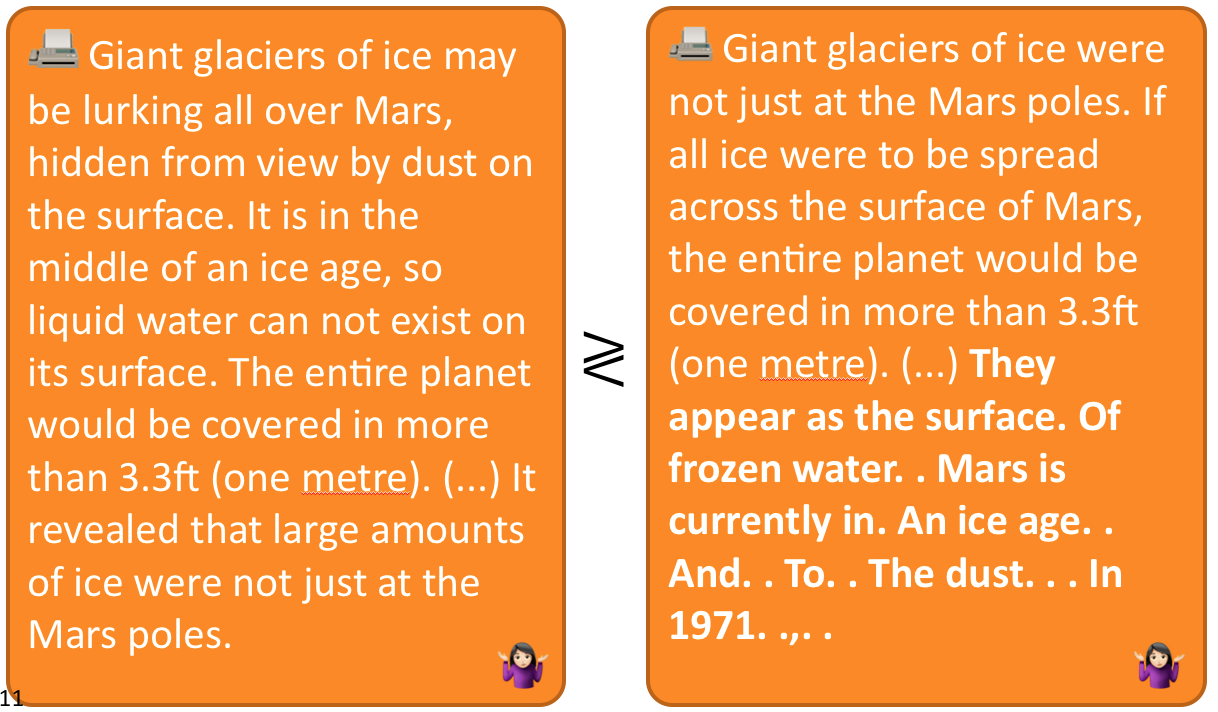
\includegraphics[width=\textwidth]{figures/example-summarization}
    \caption{\label{fig:intro:example-summarization} Text summarization. }
  \end{subfigure}
  \caption[Examples highlighting the limitations of incomplete evaluation sets]{\label{fig:intro:examples} Examples where the reference data is unable to evaluate a system's response:
  (a) Knowledge base population: here, the incomplete reference data is unable to identify that it is a true that Carrie Fisher was also an author, but not that she is a `princess'.
  (b) Open-response question answering: it is common for systems to output a paraphrase of the reference answer and thus to be judged incorrect despite reporting the right answer.
  (c) Text summarization: systems rarely produce output that is identical to the reference answer and word-overlap based similarity measures often prefer bad responses with high lexical similarity over good responses that more more lexically distinct.  
  }
\end{figure}

%\paragraph{Knowledge base Population.}
\reffig{intro:example-kbp} shows the candidate output of two KBP systems for Carrie Fisher, the late actress who played Princess Leia in the Star Wars movie franchise.
The incomplete KBP reference data only specifies that Ms.\ Fisher is an actress and thus the evaluation is unable to judge whether the system that identifies her to also be an author (which is correct) is better or worse than one that identifies her to also be a princess (which is incorrect): by default, the evaluation penalizes both decisions equally.
As a consequence, using this evaluation as an empirical guide leads researchers to avoid improvements that would identify Ms.\ Fisher as an actress.

%\paragraph{Question answering.}
Next, consider an example in question answering:
  here, the fundamental problem is that there are many ways to express the same answer (\reffig{intro:example-qa}).
It is not yet easy to automatically identify whether two phrases mean the same thing and hence fairly judge the output systems produce.
More subtly, we show that this evaluation is biased towards easier questions with short answers that are more likely to be reproduced by a system.

%\paragraph{Text summarization.}
Finally, consider the evaluation of text summarization: a system generated summary will never exactly match the one in the evaluation dataset.
A common practice in the community is to use a word-overlap based similarity score such as BLEU~\citep{papineni02bleu} or ROUGE~\citep{lin2004rouge}\@.
Unfortunately, these automatic metrics have been shown to correlate extremely poorly with human judgment~\citep{novikova2017why}.
\reffig{intro:example-summarization} shows an example of a published system that learns to game this metric by appending seemingly random words at the end of a summary.

\section{Addressing incompleteness with human feedback}
We've just seen how the incompleteness of our evaluation sets can introduce bias.
How fundamental is incompleteness?
In the setting of knowledge base population, it is possible to minimize the impact of incompleteness by exhaustively annotating a sufficiently large document collection.
We estimate that this would cost at least \$1 million; of course, any adjustment in the task definition (e.g.\ the relation schema) would require a fresh batch of annotations.
In this sense, handling incompleteness in KBP evaluation can be viewed as a prudent cost-saving measure.
On the other hand, the number of correct wordings for an answer in text summarization or open-ended question answering are nearly endless; we doubt that any amount of money would be sufficient to ameliorate the problem here.

The crux of the problem is estimating the impact of instances that are unknown to the automatic evaluation that relies on a static dataset.
We exploit the fact that the answers to these instances are obvious to humans and propose asking people for feedback \textit{on-demand} using advances in crowdsourcing. %, which has led to a number of high quality datasets~\citep{}.
In this work, we advocate moving from annotating data in batches to annotating data \textit{on-demand}.

Apart from fixing the problem of incompleteness, incorporating human feedback has several ancillary benefits.
First, it ensures that our evaluation does not diverge from the end goal.
Second, it provides \textit{qualitative} guidance to help us identify opportunities for improvements.
As an example of this latter point, in \refchap{kbpo} we show how combining human labels with statistical estimators can be used to conduct fine-grained error analysis for KBP, and in \refchap{price} we show how collecting human edits as feedback can be used for error analysis in text generation.

%Finally, the role of evaluation is two-fold: first to provide \textit{quantitative} guidance that help us empirically validate improvements to systems, and secondly \textit{qualitative} guidance to help us identify opportunities for improvements.

\section{Integrating human feedback with statistical estimators}
While human evaluation is often regarded as a gold standard for evaluation, it is also considered to be too expensive to be used as when iterating on models.
The key question this thesis tries to answer then is: can we reduce the cost of human annotation in evaluation while maintaining its fidelity?
Our core contribution is in addressing the problem of incompleteness for two extremes: problems where incompleteness is large but finite (KBP), and problems where incompleteness is truly infinite (TS and OQA).
In both settings, we hold \textit{unbiased} estimation as our bar: the methods we describe are guaranteed to produce the same results in expectation as would human evaluation.

\paragraph{Amortizing costs when incompleteness is finite.}
In settings where incompleteness is finite, it is likely that two different systems produce an overlapping set of outputs, suggesting that we may can leverage human annotations obtained for one system to evaluate another.
The key challenge is guarding against representation bias: we don't want to skew the evaluation towards a particular class of systems simply because our evaluation data came from these systems.
We tackle this problem in \refchap{kbpo} using a novel importance-reweighted estimator. We apply the estimator to evaluate KBP systems and show that we are able to reduce the cost of obtaining human annotations by a factor of 4.

\paragraph{Finding limitations when incompleteness is infinite.}
On the other end of the spectrum, in tasks like text summarization or open-ended question answering, the output produced consists of free form text: it  is extremely unlikely that two systems will ever agree on the output they produce.
Here, it seems natural to rely on some ``similarity'' measure that may allow us to match two similar, but non-identical responses.
In \refchap{price}, we derive an optimal estimator to combine such a similarity metric with human feedback based on control variates~\citep{owen2013monte}.
Our theoretical analysis allows us to characterize when it is possible to reduce human annotation costs while guaranteeing unbiasedness.
We show that for both text summarization and open-ended question answering current cost savings are modest, about 10--15\%, owing to both the poor quality of existing automatic metrics and the inherent annotator variance for these subjective tasks.

\paragraph{Beyond evaluation.}
Thus far, we have focused on the use of human feedback during evaluation.
In the \refchap{otj}, we show how human feedback can be effectively integrated \textit{at test-time}.
We consider an ``on-the-job'' setting, where our model learns as inputs arrive: we use real-time crowdsourcing to resolve uncertainty where needed and output our prediction once the model is confident.
As the model improves over time, the reliance on crowdsourcing queries decreases. 
We cast our setting as a stochastic game based on Bayesian decision theory, which allows us to balance latency, cost, and accuracy objectives in a principled way. 
Computing the optimal policy is intractable, so we develop an approximation based on Monte Carlo Tree Search.
We tested our approach on three datasets---named-entity recognition, sentiment classification, and image classification.
On the NER task we obtained more than an order of magnitude reduction in cost compared to full human annotation, while boosting performance relative to the expert provided labels.
%We also achieve a $8\%$ \fone{} improvement over having a single human label the whole set, and a $28\%$ \fone{} improvement over online learning.

%\section{Conclusions}
%Finally, in \refchap{discussion} we conclude this thesis with a discussion on the further uses of human feedback in building natural language systems.
%Our discussion touches upon possible opportunities to improve upon human evaluation as a methodology for natural language generation tasks and how human feedback provides us with a more holistic view of evaluation.
%






% In other situations, such as performing information extraction on the web, the collection of inputs that express a particular concept may itself be so varied that it is unrealistic to expect that we may cover them in a static training dataset.
% Finally, in the context of automatic text generation, the assumption that there exists a single well-defined ``correct'' output is broken.
% 
% % What happens when the data we need for learning systems is not collectible?
% 
% % We explore using human feedback in these settings.
% 




% In natural language tasks such as knowledge base population, text summarization or open-response question answering, a significant challenge is simply evaluating the performance of automated systems because of the large diversity of possible outputs.
% % ^^ Include the fact that the domain has shifted?
% Existing fully-automatic methods for evaluating these systems rely on an incomplete set of annotated references which lead to systematic biases against certain system improvements: in other words, genuinely good ideas are systematically discarded simply because of limitations in our evaluation methodology.
% As a result, human evaluation, which can be prohibitively expensive, has remained the de-facto mode of evaluation for these tasks.
% In this work, we show how one can decrease the costs of incorporating human feedback through the design of appropriate statistical estimators. 
% 
% First, we consider the setting where the output produced by systems is ``dense'', in that we expect significant overlap between the output of different systems. 
% Naively combining annotations from different systems leads to a representation bias.
% Here, we show that cost of obtaining human feedback can be significantly amortized by using a novel importance-reweighted estimator.  
% We apply this estimator to design a new evaluation methodology for knowledge base population and show that cost of evaluating precision and recall within this framework can be reduced by a factor of 4.
% 
% Next, we consider the ``sparse'' setting wherein few, if any, systems ever produce identical output.
% Traditionally, the community has relied on similarity-based automatic metrics such as BLEU or ROUGE to compare the outputs produced by different systems.
% Unfortunately, these metrics have been shown to poorly correlate with human judgment and thus introduce bias in evaluation.
% We derive an unbiased estimator that optimally combines these automatic metrics with human feedback.
% Our theoretical results allow us to characterize potential cost reductions only in terms of the tasks' subjectivity, measured by inter-annotator variance, and the automatic metrics' quality, measured by correlation with human judgments.
% On two popular natural language generation tasks, question answering and summarization, we empirically show that currently we can achieve at most a 7--13\% reduction in cost on two tasks, exposing fundamental limitations in debiasing current automatic metrics.
% 
% Finally, we show how human feedback can be incorporated into systems in real-time to deploy high-accuracy systems starting with zero training examples.
% We build systems that learn ``on-the-job'' by using human feedback to resolve uncertainty until it is confident in its predictions.
% Our key statistical idea here is to cast the problem as a stochastic game based on Bayesian decision theory, which allows us to balance latency, cost, and accuracy objectives in a principled way.
% When tested on three classification tasks---named-entity recognition, sentiment classification, and image classification--- we obtained an order of magnitude reduction in cost compared to full human annotation, while also boosting performance relative to the expert provided labels.
% 

% 
% 
% % We are used to supervised data specifying tasks, but this is a limiting perspective.
% One of the key insights of modern machine learning is that data provides a specification for otherwise fuzzy concepts like ``What is the sentiment expressed by this sentence?'', ``Is this sentence an example of hate-speech?'' or ``What semantic role does this word play in the sentence?''.
% Given a sufficiently large dataset of inputs paired with class labels, we have found models that are expressive enough to learn good definitions for these concepts.
% % TODO: Examples?
% % Sentiment (and other text) classification
% % Semantic role labeling and dependency parsing
% 
% Of course, there are many applications where this perspective of learning is insufficient.
% In many situations, one wishes to build a new system --- e.g., to do Twitter information extraction
% \citep{li2012twiner} to aid in disaster relief efforts or monitor public
% opinion --- but one does not have the luxury of time or resources to collect a ``sufficiently large'' dataset before deploying the system.
% In other situations, such as performing information extraction on the web, the collection of inputs that express a particular concept may itself be so varied that it is unrealistic to expect that we may cover them in a static training dataset.
% Finally, in the context of automatic text generation, the assumption that there exists a single well-defined ``correct'' output is broken.
% 
% % What happens when the data we need for learning systems is not collectible?
% 
% % We explore using human feedback in these settings.
% 
% % 1. What are the metaphors: vision of the future -- enabling applications -- needing to climb the ladder -- human feedback is the ladder -- how do we make it cheaper?
% % how do we effectively use 
% What tools must exist in the future in order to make effective use of the ever-expanding corpus of information available at our fingertips?
% Given that the working set memory of the average human being is only <>,
%   it is natural to expect that tools that 
% Here, information retrieval has already helped, but not enough.
% 
% Consider, for example, tools that allow us to summarize entire document troves to learn key information about the people mentioned within, tools that allow us to ask questions that synthesize information across these entire collections, and tools that can summarize articles.
% All of these applications have been actively pursued by the NLP community for many years and remain incredibly challenging.
% 
% No doubt, this is because of many many reasons, but one that we wish to explore here is the lack of a reliable evaluation methodology.
% Evaluation is the key ingredient that establishes a science and engineering.
% By establishing a ladder, we allow ourselves to climb up one step at a time to soaring heights.
% 
% In this metaphor, existing evaluation methodologies are broken ladders -- one step up indeed leads us two steps down.
% 
% 
% 
% Our goal is simple: to enable the development of systems that can effectively summarize information for us.
% 
% 
% 
% 
% Let us peer into a vision of the future for natural language processing:
%   all of the world's information is made available to us and we are able to ask systems 
% 
% % Where is it most cost-effective?
% 
% % Story 
% % 1. Picture of the future. Systems that can do X, Y, Z. 
% Let us 
% 
% % 2. Where we are now.
% % 3. What is holding us back?
% 
% 
% % 1. Field setup
% 
% For a long time, the natural language processing (NLP) community has striven to build a foundation to process language at the lexical, syntactic and semantic level.
% We have seen tremendous progress at identifying such low-level information as parts-of-speech and syntactic parses: today's systems certainly rival human performance on these tasks.
% 
% At the same time, we continue to struggle to understand basic semantics: transferring labels across domains,
% 
% We believe that a key challenge to solving these tasks is the absence of a ladder that will allow us to climb. 
% Hard to bootstrap -- here is where humans should come in.
% 
% Closing the loop: increase interaction, having machines synthesize responses for people.
% 
% [synthesis evaluation] --- [adaptation (also in tandem)]
% 
% what are the classification problems?
% - sentiment classification
% - abuse classification
% - intent classification
% - 
% 
%   We
% A common pattern for most of these problems is that they are classification problems.
% 
% By no means have all the key problems of natural LP -- the challenges of deep text understanding truly remain.
% As we solve these problems, 
% 
% 
% 
% In some sense, we have followed a Turin model of artificial intelligence: we set up tests and compare ourselves with a human == can we do as well as a person?
% In the world of generation this is b no means as easy to define.
% Indeed the past is littered with attempts and waves of progress.
% 
% What new tool do we have for this now?
% Crowdsourcing is thy name.
% 
% 
% The field of natural language processing has advanced to the degre
% 
% How do systems co-evolve with humans?
% People get to train on the job to learn what to do.
% We can enable this for machines too with OTJ.
% 
% % Over the last X years, we've basically solved classification.
% % The new frontier is generation, with new interest in many different tasks.
% 
% % 2. The problem: evaluation
% % A dogged problem for this field is evaluation.
% % Evaluation has been studied extensively for a long time.
% % Some of the limitations.
% 
% % 3. The enabler: crowdsourcing
% % Recent past, crowdsourcing has really enabled us to change the way we collect data and annotations.
% % At no earlier point could we interactively collect annotations.
% % But expensive.
% 
% % 4. The solution: statistical estimation.
% % Revisit evaluation, we find that there are problems with cost
% % Different settings require different solutions.
% % Sparse vs Dense.
% 
% % 5. More problems: on-the-job.
% 
% Placeholder.
% 
